\chapter{Evaluation}

To evaluate the new file system on \osv{}, we conducted tests comparing it
with the other available file systems, as well as with \viofs{} on linux,
when that was applicable. The tests include three scenarios, as detailed in
this chapter: a synthetic benchmark or microbenchmark, a startup time test and
an application benchmark.

\section{Methodology}

All the tests were performed on a personal computer with the specifications in
table \ref{tab:host-specs}, while table \ref{tab:guest-specs} includes the
specifications of the \osv{} and linux guests. As for their execution, we
note the following:
\begin{itemize}
    \item All tests used a temporary file system (tmpfs) % ref https://www.kernel.org/doc/html/v5.8/filesystems/tmpfs.html
          on the host, for the \osv{} images as well as for the shared
          directories in the cases of \viofs{} and NFS. This was decided upon so
          that performance was independent of the host's storage devices.
    \item Dynamic CPU frequency scaling was disabled, utilizing the
          ``performance'' CPU scaling governor % ref https://www.kernel.org/doc/html/v5.8/admin-guide/pm/cpufreq.html
          on the host.
    \item The \qemu{} process was isolated from the rest (virtiofsd, perf,
          vegeta) in terms of CPU execution (CPU pinning). % ref https://man7.org/linux/man-pages/man2/sched_setaffinity.2.html
          Specifically, \qemu{} was dedicated as many CPU cores as the guest's
          CPUs, whereas the other aforementioned processes were restricted to
          the rest of the cores available. The reason behind this was to
          minimize interference between them which could affect the results.
    \item For measuring CPU usage we chose perf \cite{perf} (version
          5.7.g3d77e6a8804a), the \texttt{perf stat} command with the
          ``task-clock'' perf event to be precise. We used this to acquire
          measurements for the \qemu{} process, virtiofsd, the vhost kernel
          thread \cite{stefanha:vhost} and the NFS kernel threads, each where
          applicable.
    \item All tests were repeated 10 times, of which we later present the
          mean value and standard deviation of the measurements. In \osv{}'s
          case every repetition consisted of a fresh VM instantiation, whereas
          in linux all repetitions were performed in a common virtual machine
          execution.
    \item Virtiofsd was run with its cache mode disabled (\texttt{cache=none})
          and a single thread (\texttt{-{}-thread-pool-size=1}). The latter was
          selected because it led to slightly more consistent measurements,
          though without improved performance, as was mentioned in a \viofs{}
          mailing list discussion%
          \footnote{\url{https://www.redhat.com/archives/virtio-fs/2020-September/msg00068.html}}.
    \item For running \osv{} we made use of the helper script (scripts/run.py)
          it provides, after modifying it in order to orchestrate execution of
          all other tools (virtiofsd, perf, vegeta). As for the virtual
          machine's networking, \qemu{}'s tap backend % ref https://www.qemu.org/docs/master/system/invocation.html#hxtool-5
          was used, with vhost enabled, with a static IP address granted to the
          VM.
    \item For the NFS server, the respective linux implementation was used on
          the host. All tests were carried out with NFS version 3, since version
          4 was not functional on the \osv{} side. Readahead on the NFS client
          (libnfs), which is equivalent to the chunk size in our implementation
          of the DAX window manager, was set to 2 MiB.
\end{itemize}

\begin{table}
    \centering
    \begin{tabular}{ |c|c| }
        \hline
        CPU & Intel Core i7-6700 @3.4GHz \\
        \hline
        Memory & 2\(\times\)8 GiB @2666MHz \\
        \hline
        Swap & No \\
        \hline
        linux kernel & 5.8.13-arch1-1 \\
        \hline
        \qemu{} & 5.1.50 @ c37a890d12e57a3d28c3c7ff50ba6b877f6fc2cc \cite{virtiofs:qemu} \\
        \hline
    \end{tabular}
    \caption{Specifications of the host.}
    \label{tab:host-specs}
\end{table}

\begin{table}
    \centering
    \begin{tabular}{ |c|c| }
        \hline
        CPUs & 4 \\
        \hline
        Memory & 4 GiB \\
        \hline
        DAX window & 4 GiB \\
        \hline
        \osv{} & 5372a230ce0abf0dc72e92ec1116208145e595c5 \cite{osv-repo} \\
        \hline
        linux kernel & 5.8.0-rc4-33261-gfaa931f16f27 \cite{virtiofs:linux} \\
        \hline
    \end{tabular}
    \caption{Specifications of the guests.}
    \label{tab:guest-specs}
\end{table}

\section{Microbenchmark}

\subsection{Description}

For measuring the file system's performance we used the flexible I/O tester
(fio) \cite{fio} in its 3.23 version. In order for it to run on \osv{}, two
modifications were necessary%
\footnote{All modifications can be found in the ``fio-3.23-osv'' tag of the git
repository at \url{https://github.com/foxeng/fio}.}
in addition to the appropriate arguments to fio's configure script, to disable
features not provided by \osv{}. We note that the exact same executable (with
the above disabled) was used in linux as well.

The comparison includes ZFS, rofs, ramfs, \viofs{} (with and without the DAX
window and with a ramfs root file system) and NFS on \osv{}, \viofs{} (with
and without the DAX window and with an ext4 root file system) on linux, as
well as tmpfs on the host, which we include as a baseline. Specifically for the
testing process:
\begin{itemize}
    \item In all cases except ramfs, the fio test files have been layed out in
          advance and subsequently placed in the appropriate location (virtual
          disk or shared directory). We chose this approach despite fio being
          able of laying out the files dynamically at run time since some of the
          file systems are read-only. Because ramfs is restricted as to the size
          of individual files in its image, the test files are generated at run
          time in its case.
    \item We examine two cases as to the test files:
          \begin{itemize}
              \item A single, large file (1 GiB).
              \item Multiple (10) smaller files (80-100 MiB). We note that in
                    all tests the files are identical (each respective file is
                    of the same size).
          \end{itemize}
          In both cases the overall file size does not exceed 1 GiB, in part due
          to this being limited by the guest's memory for rofs and ramfs, as
          well as the DAX window for \viofs{} with DAX.
    \item We examine two cases as to the file reading pattern: serial
          (\texttt{rw=read}) and random (\texttt{rw=randread}). % ref https://github.com/foxeng/osv/tree/virtiofs-tests/modules/fio/tests
    \item In all cases there is a single thread reading (\texttt{numjobs=1}).
    \item On linux, for the automation of the tests we relied on Vivek
          Goyal's relevant helper%
          \footnote{commit hash 8c99f50c878cb39db76abec7e0882fd83c99f4b3}
          \cite{virtiofs-tests}. This invalidates the page, inode and dentry
          caches using a sysctl (/proc/sys/vm/drop\_caches) % ref https://www.kernel.org/doc/html/latest/admin-guide/sysctl/vm.html
          before each fio run.
    \item In the case of linux (guest and host), there was no CPU usage
          measurement, since that was deemed unworthy, given the difference in
          nature from \osv{} (general-purpose OS vs unikernel).
\end{itemize}

\subsection{Results}

\begin{figure}
    \begin{minipage}[c][\textheight]{\textwidth}
        \begin{subfigure}[c][0.5\textheight]{\textwidth}
            \caption{Throughput}
            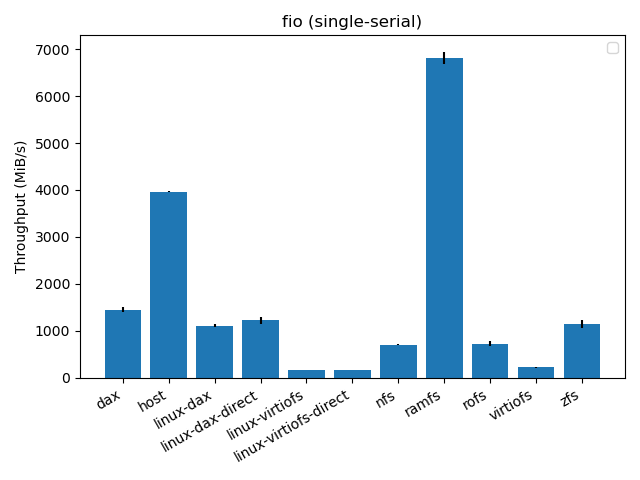
\includegraphics[width=\textwidth]{fio-single-serial-tput}
            \label{fig:fio-single-serial-tput}
        \end{subfigure}
        \begin{subfigure}[c][0.5\textheight]{\textwidth}
            \caption{CPU usage}
            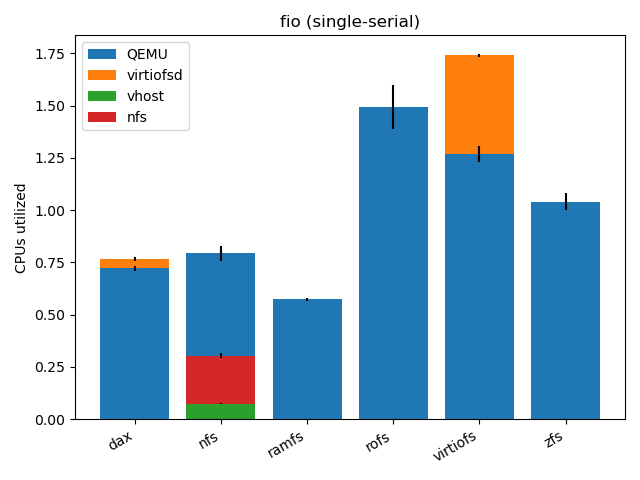
\includegraphics[width=\textwidth]{fio-single-serial-cpu}
            \label{fig:fio-single-serial-cpu}
        \end{subfigure}
        \caption{fio, single file, serial reading}
        \label{fig:fio-single-serial}
    \end{minipage}
\end{figure}

\begin{figure}
    \begin{minipage}[c][\textheight]{\textwidth}
        \begin{subfigure}[c][0.5\textheight]{\textwidth}
            \caption{Throughput}
            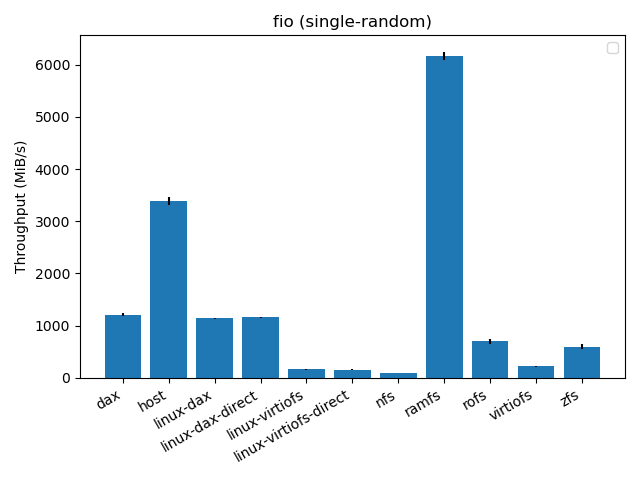
\includegraphics[width=\textwidth]{fio-single-random-tput}
            \label{fig:fio-single-random-tput}
        \end{subfigure}
        \begin{subfigure}[c][0.5\textheight]{\textwidth}
            \caption{CPU usage}
            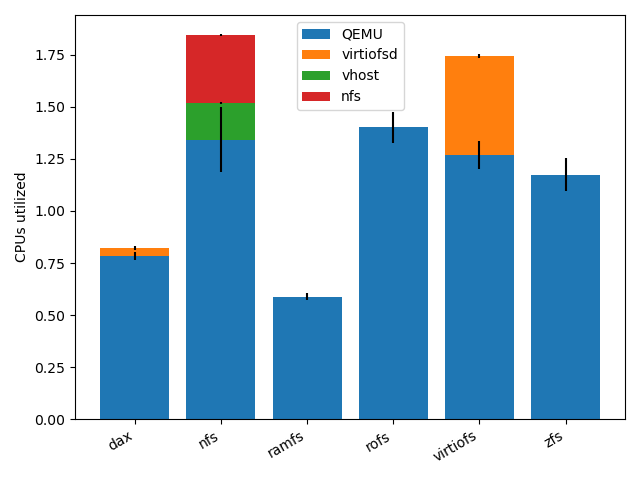
\includegraphics[width=\textwidth]{fio-single-random-cpu}
            \label{fig:fio-single-random-cpu}
        \end{subfigure}
        \caption{fio, single file, random reading}
        \label{fig:fio-single-random}
    \end{minipage}
\end{figure}

\begin{figure}
    \begin{minipage}[c][\textheight]{\textwidth}
        \begin{subfigure}[c][0.5\textheight]{\textwidth}
            \caption{Throughput}
            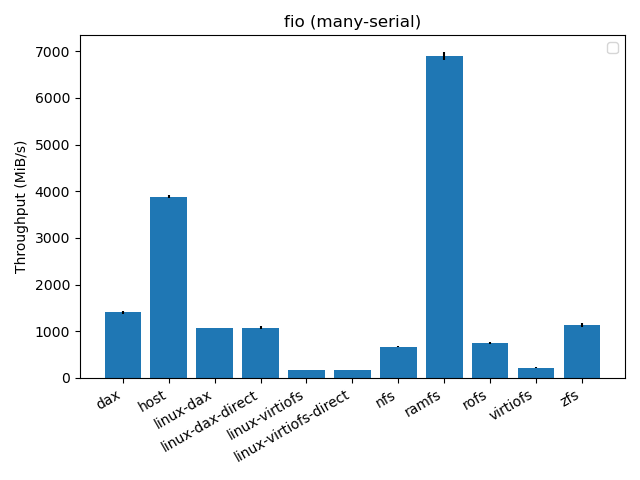
\includegraphics[width=\textwidth]{fio-many-serial-tput}
            \label{fig:fio-many-serial-tput}
        \end{subfigure}
        \begin{subfigure}[c][0.5\textheight]{\textwidth}
            \caption{CPU usage}
            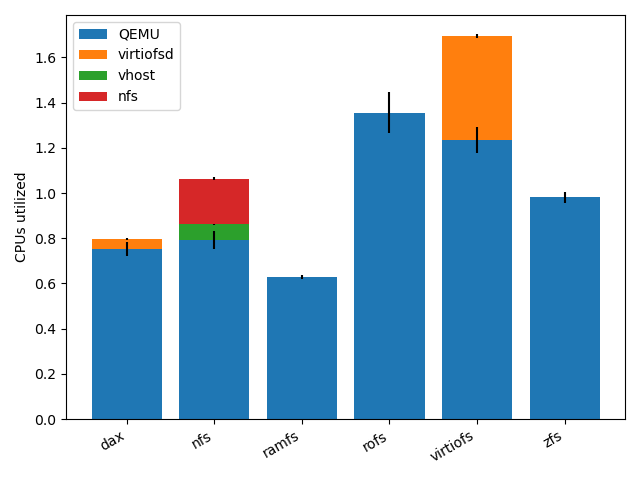
\includegraphics[width=\textwidth]{fio-many-serial-cpu}
            \label{fig:fio-many-serial-cpu}
        \end{subfigure}
        \caption{fio, multiple files, serial reading}
        \label{fig:fio-many-serial}
    \end{minipage}
\end{figure}

\begin{figure}
    \begin{minipage}[c][\textheight]{\textwidth}
        \begin{subfigure}[c][0.5\textheight]{\textwidth}
            \caption{Throughput}
            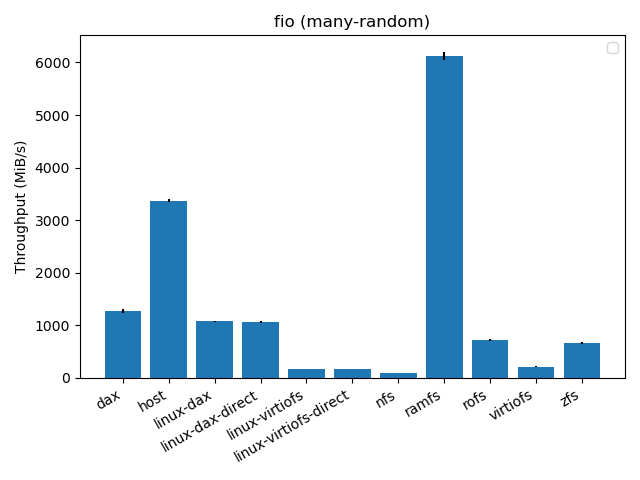
\includegraphics[width=\textwidth]{fio-many-random-tput}
            \label{fig:fio-many-random-tput}
        \end{subfigure}
        \begin{subfigure}[c][0.5\textheight]{\textwidth}
            \caption{CPU usage}
            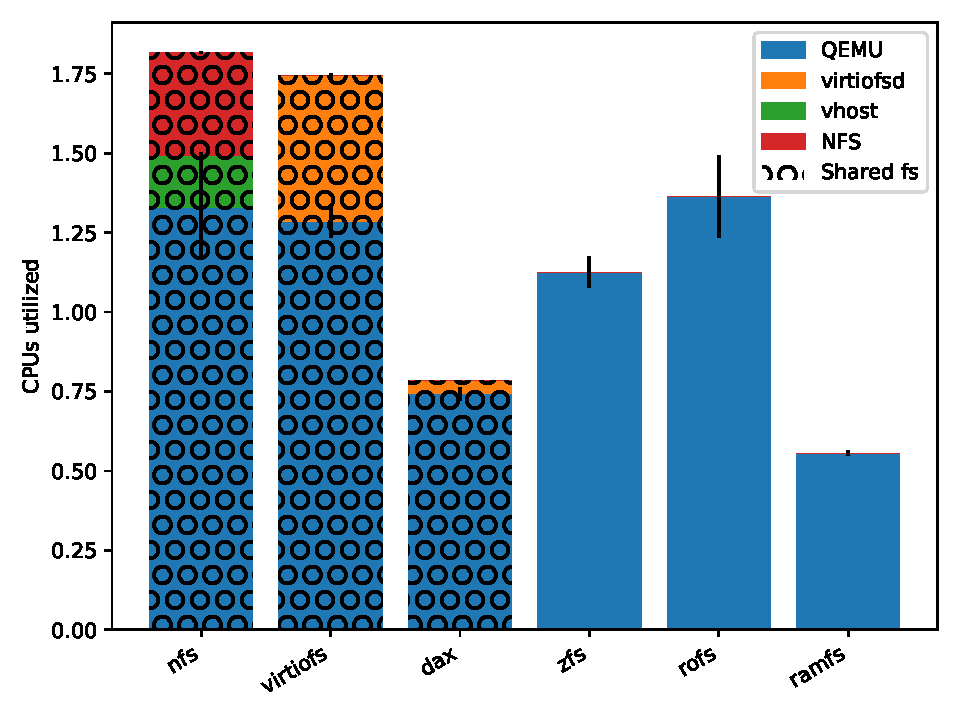
\includegraphics[width=\textwidth]{fio-many-random-cpu}
            \label{fig:fio-many-random-cpu}
        \end{subfigure}
        \caption{fio, multiple files, random reading}
        \label{fig:fio-many-random}
    \end{minipage}
\end{figure}

% tst   OSv    Linux
%  s-s: 220  - 170  (virtio-fs)
%       1450 - 1108 (DAX)
%       707         (NFS)
%  s-r: 217  - 163  (virtio-fs)
%       1212 - 1142 (DAX)
%       85          (NFS)
%  m-s: 219  - 166  (virtio-fs)
%       1402 - 1071 (DAX)
%       668         (NFS)
%  m-r: 215  - 166  (virtio-fs)
%       1269 - 1081 (DAX)
%       85          (NFS)
% mean: 217  - 166  (virtio-fs)
%       1333 - 1100 (DAX)
%       386         (NFS)

As we can see in fig. \ref{fig:fio-single-serial} through
\ref{fig:fio-many-random}, the highest throughput is achieved by ramfs on
\osv{}, even higher than that of tmpfs on the host. This is so because, with the
data in memory the virtualization overhead is minimized, while the simpler
file system implementation and lack of mode switches due to system calls on
\osv{} seem to make the difference. Virtio-fs with DAX offers the next best
performance on \osv{}, in all cases, also having the lowest impact in terms of
processing resources consumed, again after ramfs.

Focussing on \viofs{} and comparing between \osv{} and linux, we discern
consistent behavior in all cases: in both operating systems the DAX window
outperforms \viofs{} without it, by a large margin (\(> 6 \times\) throughput),
while on \osv{} we notice \(20 - 30 \%\) better performance than linux. The
latter is expected, in part due to the simpler, hence more efficient \osv{}
implementation, supporting a lot less features and in part due to the relative
advantages of a unikernel.

We owe a mention to the comparison between \viofs{} and NFS, the only shared
file systems on \osv{}. Here \viofs{} with the DAX window leads in performance,
with NFS following and \viofs{} without DAX trailing, in the serial read tests.
As seen in table \ref{tab:fio-virtiofs-nfs}, the pattern is different in the
random read tests, with NFS performing the worst, both in terms of throughput
and of CPU usage. It seems thus to have been much more adversely impacted than
\viofs{} by the change in the access pattern which adds pressure to the
speculation and caching mechanisms of all file systems.

\begin{table}
    \centering
    \begin{tabular}{ |c|c|c|c| }
        \hline
        pattern & \viofs{} & NFS & \viofs{} DAX \\
        \hline
        serial & 1.0 & 3.1 & 6.5 \\
        random & 1.0 & 0.4 & 5.7 \\
        \hline
    \end{tabular}
    \caption{Normalized fio throughput, \viofs{} and NFS on \osv{}.}
    \label{tab:fio-virtiofs-nfs}
\end{table}

\section{Startup time}

\subsection{Description}

In order to evaluate startup time on \viofs{} we chose an application of those
already ported to \osv{} as examples \cite{osv-apps}. Specifically, we selected
spring-boot-example, a simple web application from \cite{spring-boot-examples},
built using the spring boot framework, % ref https://spring.io/projects/spring-boot
in its 2.3.4 version.%
\footnote{All changes made for our tests can be found in the ``virtio-fs-tests''
tag of the git repository at \url{https://github.com/foxeng/osv-apps}.}
As for the Java runtime, we chose openjdk8-zulu-full, again from \osv{}'s
application repository. This application was qualified as representative of
stateless web applications, prime examples of the class suitable for deployment
as unikernels in the cloud.

All \osv{} file systems usable as root file systems participated in this set of
tests: ZFS, rofs, ramfs and \viofs{}. The testing process consisted of booting
\osv{} with each file system as the root file system. This was then left to run
for a reasonable amount of time (a few seconds), during which the application
reached its fully initialized state and subsequently terminated by the test
orchestration mechanism (script), by terminating the \qemu{} process.

\subsection{Results}

Figure \ref{fig:startup-app} depicts a breakdown of the total startup time:
\begin{description}
    \item[OSv boot] is the system's boot time, i.e. the application-independent
          part.
    \item[Root fs mount] involves the root file system mount time and the time
          to pivot ``root'' (/) to it. We note that this is also a stage of the
          above, but here it is extracted from it and examined separately.
    \item[Application] encompasses the time taken for the application's
          initialization, as reported by it.
\end{description}

\begin{figure}
    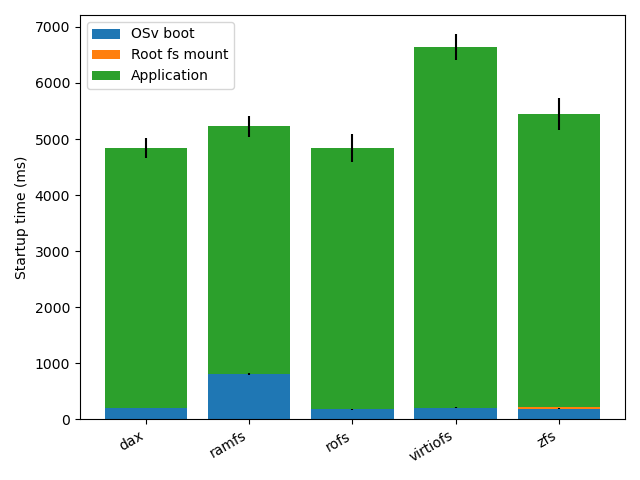
\includegraphics[width=\textwidth]{startup-app}
    \caption{Spring boot example, startup times.}
    \label{fig:startup-app}
\end{figure}

% fs        total time
% ZFS       5452
% rofs      4838
% ramfs     5226
% virtio-fs 6642
% DAX       4844

As made clearer in table \ref{tab:startup-total}, in terms of total startup
time, \viofs{} without the DAX window is inferior to the rest, with \viofs{}
with the DAX window being the best performer along rofs (ramfs and ZFS are
slightly slower).

\begin{table}
    \centering
    \begin{tabular}{ |c|c|c|c|c| }
        \hline
        ZFS & rofs & ramfs & \viofs{} & \viofs{} DAX \\
        \hline
        1.13 & 1.00 & 1.08 & 1.37 & 1.00 \\
        \hline
    \end{tabular}
    \caption{Normalized total spring-boot-example startup time on \osv{}.}
    \label{tab:startup-total}
\end{table}

As far as mount time is concerned, it is virtually negligible (\(<2\%\) of
\osv{}'s boot time) for all file systems with the exception of ZFS. In its case,
mount time takes up roughly \(14\%\) of the system's boot time, as expected
given the relative complexity of this file system, which translates to a longer
initialization procedure.

Finally, it is worth mentioning the noticeably increased \osv{} boot time with
ramfs. This can be justified, considering that in the case of ramfs, the root
file system matches the boot file system (in \osv{} terms, what linux calls
initramfs). This is part of the ELF object containing the kernel, which is
uncompressed and loaded during the early boot stages \cite{osv-wiki:early-boot},
in a process with throughput limited due to the restricted initial environment
when booting from BIOS on the x86 architecture. Hence, when in the case of
ramfs, this ELF object is up to an order of magnitude larger than in the rest,
this is responsible for the increase in boot time. Of course, here we have
abused ramfs, which is not destined for such large images.

\section{Application benchmark}

\subsection{Description}

To evaluate \viofs{} in terms of a complete, real-world application we again
turned to the field of stateless applications in the context of the cloud,
choosing a static web server scenario. Specifically, we used nginx \cite{nginx}
(in its 1.19.2 version), one of the most popular free - open source web servers,
also available in the collection of \osv{} applications.%
\footnote{All changes made for our tests can be found in the ``virtio-fs-tests''
tag of the git repository at \url{https://github.com/foxeng/osv-apps}.}

This set of tests included all \osv{} file systems (in the case of \viofs{},
ramfs was used as the root file system), except NFS which led to test failure.
Specifically, while the server was handling the first request, after sending
few initial response data, the whole process stopped and the guest seemed to
``freeze''. This was found to not be caused by nginx, since the same behavior
was displayed using lighttpd (also included in the ``osv-apps'' collection)
instead. Further investigation is warranted to pinpoint and possibly fix the
cause, which from experience seems like a deadlock, possibly in the NFS
implementation or \osv{}'s network stack.

The files exposed by the web server were 10 in total, ranging in size from
roughly 500 KiB to 12 MiB. Each respective file's size was constant throughout
all tests.

For conducting the tests, in the form of HTTP load tests, we used vegeta
\cite{vegeta} on the client side, a popular tool for this purpose, in its 12.8.3
version. The testing process (automated by the orchestration script) was:
\begin{enumerate}
    \item First of all the \osv{} guest was started, given an one second time
          frame to complete initialization of the nginx server.
    \item Vegeta was launched on the host, configured to generate HTTP 1.1 GET
          requests for all of the server's files, with the maximum rate
          possible, using 20 ``workers'' and up to 4 CPUs, with TCP connection
          keepalive on.
    \item After ten seconds vegeta concluded its work and terminated, at which
          point the automation mechanism also terminated the guest through the
          \qemu{} process.
\end{enumerate}

\subsection{Results}

\begin{figure}
    \begin{minipage}[c][\textheight]{\textwidth}
        \begin{subfigure}[c][0.5\textheight]{\textwidth}
            \caption{Requests per second}
            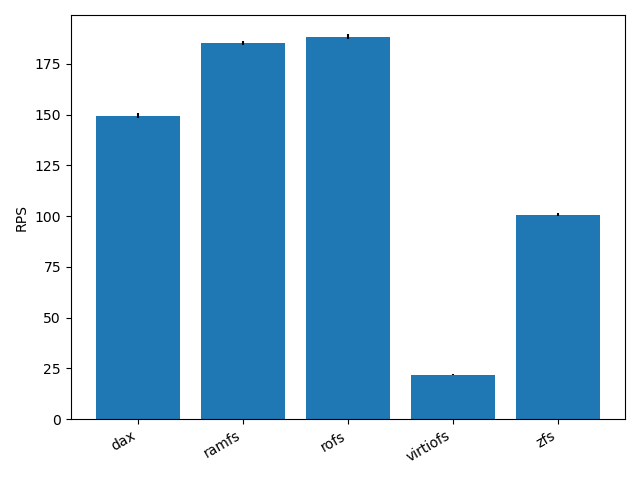
\includegraphics[width=\textwidth]{nginx-rps}
            \label{fig:nginx-rps}
        \end{subfigure}
        \begin{subfigure}[c][0.5\textheight]{\textwidth}
            \caption{CPU usage}
            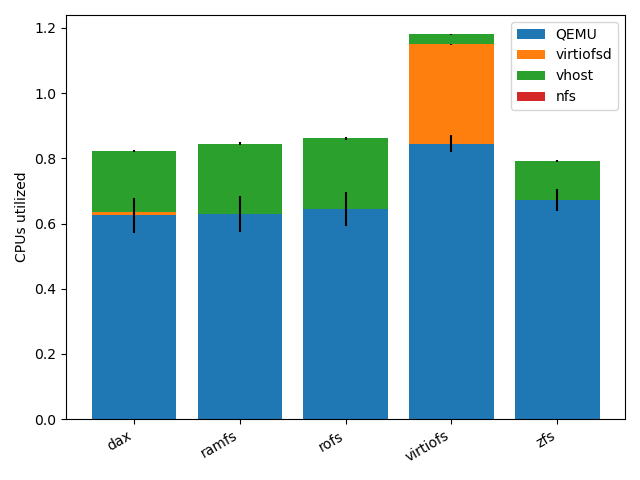
\includegraphics[width=\textwidth]{nginx-cpu}
            \label{fig:nginx-cpu}
        \end{subfigure}
        \caption{nginx HTTP load test}
        \label{fig:nginx}
    \end{minipage}
\end{figure}

% fs        rps
% ZFS       100
% rofs      188
% ramfs     185
% virtio-fs 150
% DAX       22

As we see in fig. \ref{fig:nginx-rps}, \viofs{} with the DAX window falls short
of rofs and ramfs (which lead) by \(\sim 20\%\) in terms of throughput (requests
serviced per second). Given its CPU usage is marginally lower than that of the
other two, this difference calls for further future investigation through
profiling, with focus on the \viofs{} with DAX read datapath on \osv{} as the
primary suspect.

As one could expect in this use case, \viofs{} without DAX trails behind all
other file systems by a large margin. This is down to it not making use of any
form of caching, such that each read operation involves exiting and processing
in the host (indicated by the high CPU usage). These operations are very
frequent, amplifying the effects of this overhead.
